\subsection{Attribution stability and physical consistency}\label{sec:res_shap}
Figure~\ref{fig:shap} summarises Experiment~3; its interpretation is given in Section~\ref{sec:disc}. Event-specific models agree only moderately on predictor importance (mean pairwise Spearman correlation 0.42 for GBM and 0.31 for PC-GBM). This is well above the agreement expected between random importance rankings (95th percentile 0.09), but far from consistent. Grouping the correlated predictors gives a more stable picture: for GBM, terrain variables account for 44--73\% of the mean absolute attribution, ground motion (PGA, PGV) for 24--41\% and Newmark displacement for 0.5--28\% in individual events. Maximum local slope, PGA, Newmark displacement and PGV are the most important predictors on average. Increasing PGA and PGV by 10\% lowered the predicted probability in a mean of 26\% of held-out cells for the transferred GBM and 43\% for the global LR, and in none for the constrained models.

\begin{figure*}[t]\centering
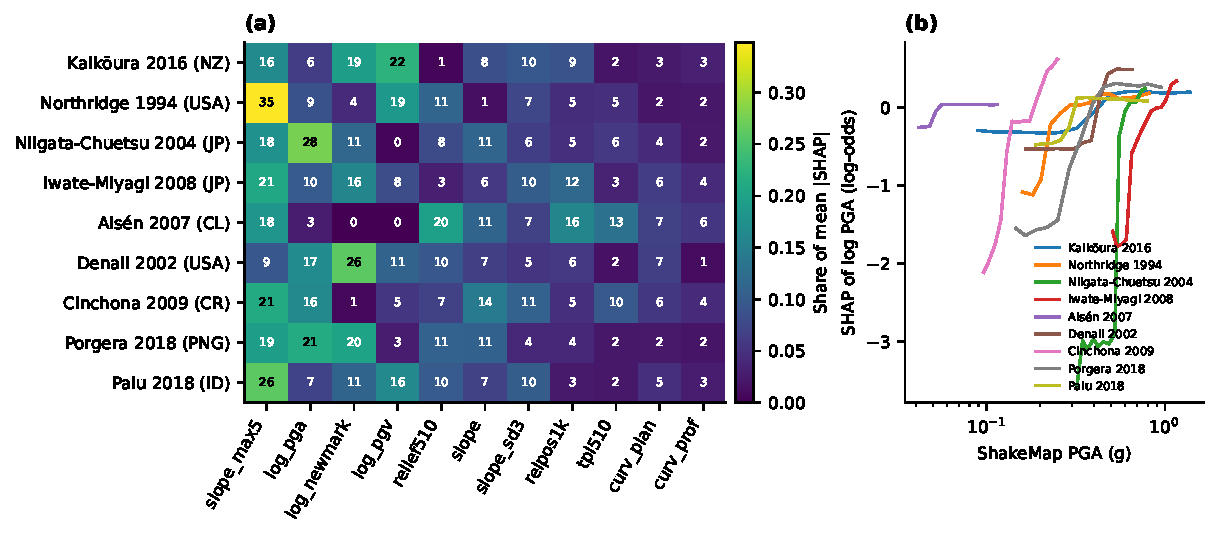
\includegraphics[width=\textwidth]{fig6_shap.pdf}
\caption{TreeSHAP attributions of event-specific PC-GBM models. (a) Share of the mean absolute SHAP value of each predictor (\%) for each event; predictors ordered by mean importance. (b) SHAP dependence of $\log_{10}$PGA (binned medians) for each event: the response is monotone in all events, but the PGA at which it rises differs by almost an order of magnitude.}\label{fig:shap}
\end{figure*}
